\documentclass[10pt,a4paper]{article}
\usepackage[utf8]{inputenc}
\usepackage[english]{babel}
\usepackage{bm}
\usepackage{ragged2e}
\usepackage{amsmath}
\usepackage{physics}
\usepackage{amsfonts}
\usepackage{amssymb}
\usepackage{float}
\usepackage{graphicx}
\begin{document}
\title{Taxonomy of serious game development approaches}
\date{}
\maketitle

\section{What is a game?}
An voluntary activity, where people interact in order to achieve some goals, within some constraints (described as game rules).
The purpose of a game is to provide tools for the players that allow them to approximate their challenging expectations. Expectations that might be provided externally, like from an instructor, or are self motivated, like being entertained.


\subsection{Formal definition of a video game}
A game is made of objects, which we call \textit{state}, whose properties change according to the progression of the time. We can represent the evolution of the state by mean of a integrator that approximates, with numeric methods, the value of state for all $T$ times of a game:
\begin{equation}\label{eq:1}
w(T) = \int_{t = 0}^{t=T} \dv{w_t}{t} dt
\end{equation}
\noindent
where $w(T)$ represents the state at time $T$. 


\paragraph{A particle} Consider a state made of a particle accelerating at  $\bar{\mathbf{a}}$ $m/s$, with velocity $v(t)$ and position $p(t)$. We can represent the just mentioned evolutions as a system of differential equations:

\begin{equation}\label{eq:2}
\left \lbrace
\begin{array}{l}
\dv{\mathbf{p}(t)}{t} = \mathbf{v}(t)\\
\dv{\mathbf{v}(t)}{t} = \mathbf{a}(t)
\end{array}
\right.
\end{equation}


\noindent
Now if we want to compute the position of the particle at time $T$ we need to update the above integrator:
\begin{equation}\label{eq:3}
\left \lbrace
\begin{array}{l}
p(T) = \int_{0}^{T} \mathbf{v}(t) dt \\
v(T) = \int_{0}^{T} \mathbf{a}(t) dt
\end{array}
\right.
\end{equation}

\noindent
The position of the particle is the result of the sum of all the velocities for all times less than $T$. All entities of the state of a game can be seen as numbers, collection of positions, collection of velocities, etc., so we can put them all in one system and the state of the game at a time $t$ consists of integrating the system at time $t$. If we expand \ref{eq:2} into:
\begin{equation}\label{eq:4}
\left \lbrace
\begin{array}{l}
\dv{\mathbf{p}(t)}{t} = \lim\limits_{dt \to 0} \dfrac{\mathbf{p}(t + dt) - \mathbf{p}(t)}{dt} = \mathbf{v}(t)\\
\dv{\mathbf{v}(t)}{t} = \lim\limits_{dt \to 0} \dfrac{\mathbf{v}(t + dt) - \mathbf{v}(t)}{dt} = \mathbf{a}(t)
\end{array}
\right.
\end{equation}

Solving the two limits in (\ref{eq:4}) requires to apply a numerical methods. We use the Euler method, which is meant for solving systems of differential equations, where $\lim\limits_{dt \to 0}$ becomes a fixed step that we call $\Delta t$.
\begin{equation}\label{eq:5}
\begin{cases}
\dfrac{\Delta \mathbf{p}}{\Delta t} = \dfrac{\mathbf{p}(t + \Delta t) - \mathbf{p}(t)}{\Delta t} = \mathbf{v}(t)\\
\dfrac{\Delta \mathbf{v}}{\Delta t} = \dfrac{\mathbf{v}(t + \Delta t) - \mathbf{v}(t)}{\Delta t} =  \mathbf{a}(t)
\end{cases}
\end{equation}

\begin{equation}\label{eq:6}
\begin{cases}
\mathbf{p}(t + \Delta t) = \mathbf{p}(t) + \mathbf{v}(t) * \Delta t\\
\mathbf{v}(t + \Delta t) = \mathbf{v}(t) + \mathbf{a}(t) * \Delta t
\end{cases}
\end{equation}

By starting from a known position we move for a small amount towards a new position which is targeted by the velocity. Of course we need an initial position for our particle so when $t=0$ we use the initial position of the particle instead of using the rule in the system.

Eventually, we can generalize the case of the particle to any object or objects of game by applying the reasoning given above and solving the proper differential equations.



\subsubsection{Numerical vs. Analytic Solutions}
The fact that we are able to model the evolution of the state by mean of a function does not mean that founding the exact solution is possible or simple. Analytical solutions solution work only for simple models. But when the model of the game becomes complex (imagine a city simulator, or a driving simulator with lots of physics) or the model is influenced by the user input, then it is not possible to identify a closed form solution. Reason why we need to use numerical methods for solving the equations such the Euler method, where the initial values are the initial state and the update describes the changes of the state over a short amount of time. Of course it is an approximation, but at least we manage to get very close to a closed form solution.

\subsection{Video game}
Within the panorama of games we find video games. A video game is a specialized kind of game where the interaction is carried out by mean of electronic devices. Precisely a video game, from now on a \textit{game}, is a program which indefinitely interacts with hardware components. Hardware components take care of: updating the memory, displaying the game entities, reading the input, etc.


\subsection{Structure of a video game}
A video game, from now on a game, is a real time simulation whose \textit{state}, made of objects, can be seen as an intractable object. \textit{Interactions} that are carried out with respect to a discrete \textit{time flow}. The discrete reason is explained by the fact that interaction with hardware components require some time. \footnote{Every increment in the state should indeed take into consideration the difference in time between now and the last time we interacted with the components.} Interactions are implemented/coded within a so called \textit{game loop} (or main loop). The game loop keeps interacting the hardware components (those components that represent the state or might change it) and at the end of each loop a new state of th game is achieved. The goal of the game is to display the game objects and to apply all interactions (from now we describe them all under the keyword update). Each complete sequence of interactions of the game loop is \textit{frame}. Updating the state of game with respect to intervals of time might seem that we loose precision, since one could argue that we might miss some information between two frames. But games exhibit some sorting of dithering in their behavior, which means that difference in the state between two consecutive frames are very small and similar. Of course as long as the frame is small\footnote{60 frames per second are a good approximation}. 







 
Science has provided a high-level representation of a game. We can represent the state of a game by mean of differential . In this representation a game can be seen as .... 



A video game:

Issue:
Mismatch between high-level and hardware representation!

\begin{figure}[H]
\centering
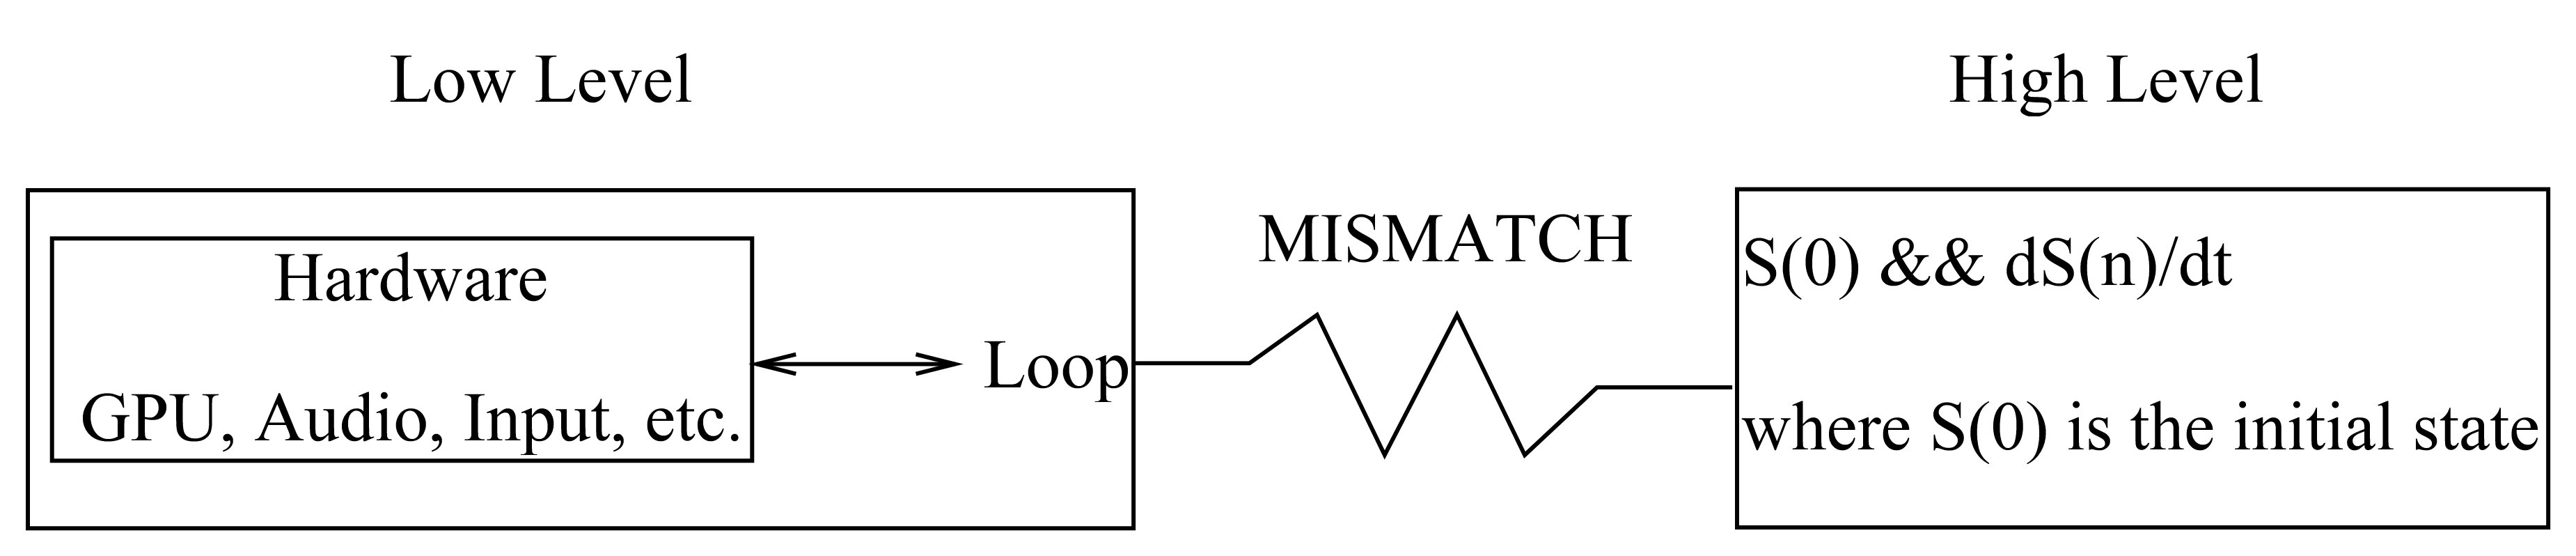
\includegraphics[scale=0.5]{games_description.png}
\caption{Game formalization (overview)}\label{game_description}
\end{figure}

In what follow we discuss how the community try to solve such mismatch my mean of tools and languages.

\section{Game development}
\begin{itemize}
\item Research in game development tries to solve the gap/mismatch between the low level constraints and the high level description of a game descried in Section \ref{section_introduction}
\item \textbf{How?} Historically a hierarchy has come to life, which is described by the picture below:
\end{itemize}

\begin{figure}[H]
\centering
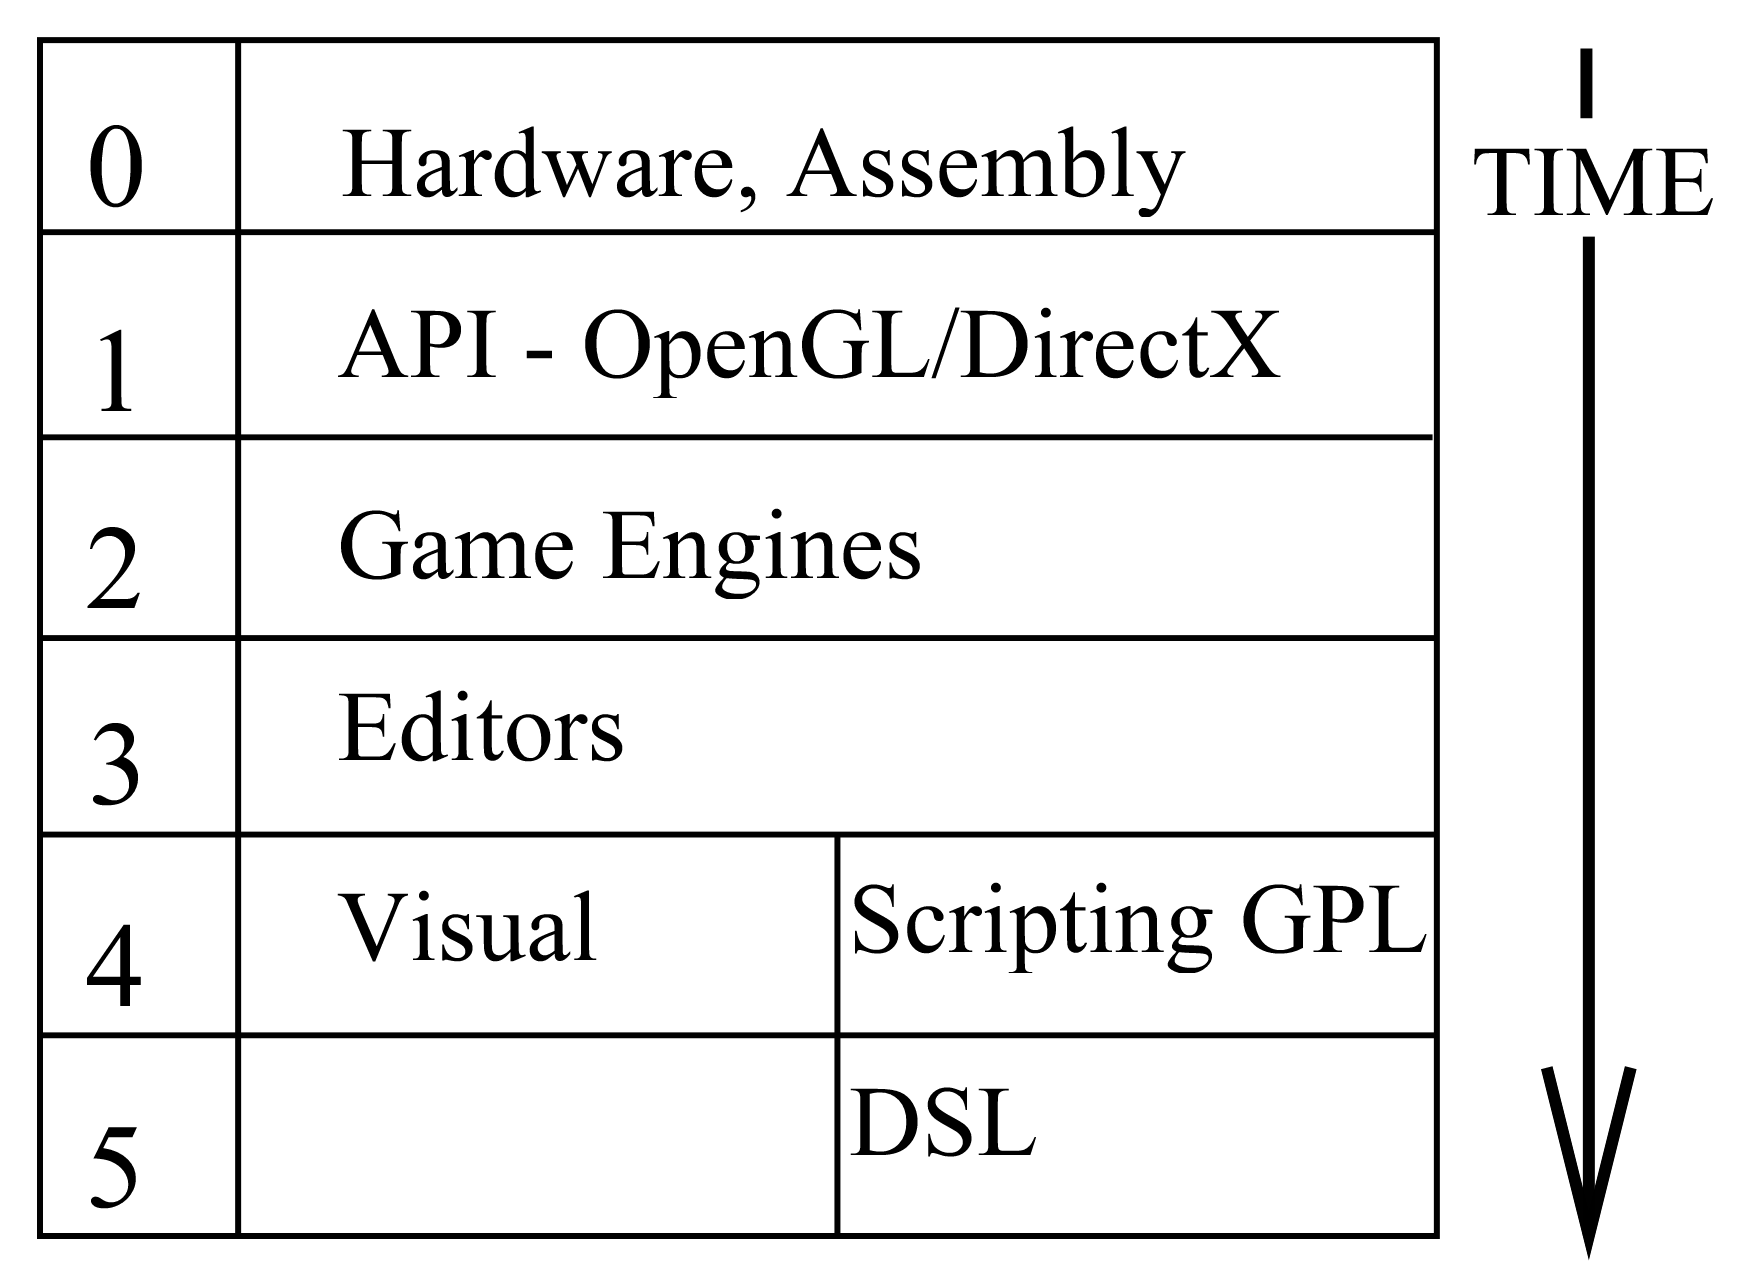
\includegraphics[scale=0.5]{game_development_evolution.png}
\caption{Game development tools evolution}\label{game_dvelopment}
\end{figure}

\subsection{Hardware} introduction, examples (assembly games), pros, and issues
\subsection{Multimedia API} introduction, examples (DirectX, OpenGL), pros, and issues
\subsection{Engines} introduction, examples (Ogre, XNA, UnityEngine), pros, and issues
\subsection{Editors} introduction, examples (UnityEditor, UnrealEngine), pros, and issues
\subsection{Visual + GPL} introduction, examples(GameMaker,RPGmaker), pros, and issues
\subsection{DSL} introduction, examples(Casanova), pros, and issues

\section{Research questions?}
For example: 
\begin{itemize}
\item To what extent a game should be designed around the domain of games and what are the requirements
\item To what extent game development would benefit from the integration of DSLs into the development processes and to what level of abstraction
\item ...
\end{itemize}
\end{document}